\section{Results}
\subsection{Corrected crowd pose evaluation}
Table~\ref{tab:pose} and Fig.~\ref{fig:pose} report the corrected CPU study. Baseline accuracy is 77.0\%, reliability 78.1\%, interactions 78.6\%, and combined 74.7\%. The interaction variant has the highest mean accuracy among these four models, with macro-F1 0.782. Reliability has a slightly higher mean ROC-AUC than interactions, so the ranking depends on the metric as well as the selected threshold. The combined variant does not improve the baseline despite its additional channels.

The motion logistic control reaches 75.1\% and the quality-only control 77.6\%. The latter is competitive without access to joint trajectories. This establishes that aggregate estimator-related information can predict supplied labels in this corpus. It does not identify whether density, scene, camera conditions, or another correlated property causes that performance. The controls' different architectures and fitting procedures also limit direct comparisons of representation capacity.

\begin{table}[t]
\caption{Corrected CPU crowd results. Accuracy is in percent. The spread is descriptive fold/seed standard deviation.}
\label{tab:pose}\centering
\begin{tabular}{lrrrr}
\toprule
Model & Fits & Accuracy & F1 & AUC\\
\midrule
Baseline & 15 & 77.0 $\pm$ 4.7 & 0.765 & 0.856\\
Reliability & 15 & 78.1 $\pm$ 6.1 & 0.777 & 0.862\\
Interactions & 15 & 78.6 $\pm$ 5.6 & 0.782 & 0.851\\
Combined & 15 & 74.7 $\pm$ 5.9 & 0.736 & 0.858\\
Motion linear & 5 & 75.1 $\pm$ 5.3 & 0.748 & 0.798\\
Quality only & 5 & 77.6 $\pm$ 6.1 & 0.773 & 0.861\\
\bottomrule
\end{tabular}
\par\smallskip\parbox{\columnwidth}{\footnotesize F1 denotes macro-F1. TCNs have 15 fits per variant; deterministic controls have five fits. Dependent runs do not provide confidence intervals.}
\end{table}

\begin{figure}[t]
\centering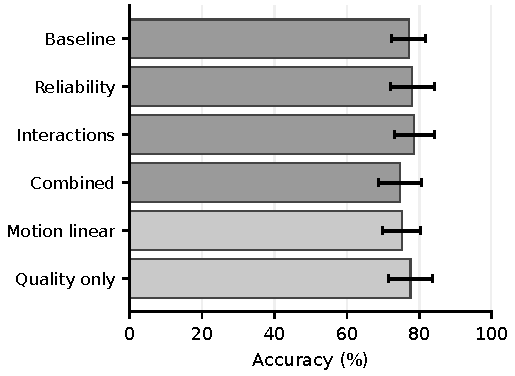
\includegraphics[width=\columnwidth]{figures/pose_results.pdf}
\caption{Corrected CPU crowd accuracy. Error bars summarize descriptive fold/seed variation for TCNs and fold variation for deterministic controls. They are not confidence intervals.}
\label{fig:pose}
\end{figure}

\subsection{Matched centering and coverage changes}
The paired centering study gives interaction accuracy 76.5\% under the legacy origin and 78.6\% under the corrected origin, an increase of 2.18 percentage points calculated from unrounded means. Reliability increases by 0.95 points. Baseline decreases by 0.54 points and combined decreases by 0.27 points (Table~\ref{tab:center}). The unchanged motion and quality controls reproduce the same held-out scores and decisions across the matched CPU studies.

These results support treating origin construction as a material implementation choice. They do not show that every pose model benefits from interpolation or that an interaction improvement transfers externally. Dependent paired runs and descriptive variation do not establish statistical significance. The correction also retains an offline dependence on complete observed segments.

\begin{table}[t]
\caption{Matched CPU centering comparison. Changes use unrounded source values and percentage points (pp).}
\label{tab:center}\centering
\begin{tabular}{lrrr}
\toprule
Variant & Legacy & Corrected & Change\\
\midrule
Baseline & 77.6\% & 77.0\% & -0.54 pp\\
Reliability & 77.1\% & 78.1\% & +0.95 pp\\
Interactions & 76.5\% & 78.6\% & +2.18 pp\\
Combined & 75.0\% & 74.7\% & -0.27 pp\\
\bottomrule
\end{tabular}
\end{table}

The earlier explicit-coverage GPU ablation leaves three variant mean accuracies unchanged and reduces interaction accuracy by 0.14 percentage points. Accuracy ties can contain changed decisions. Other masks and detection-related channels remain available, so the ablation does not remove the predictive quality signal demonstrated by the aggregate control. Its legacy-feature GPU values are retained separately from the matched corrected CPU results.

\subsection{Input controls}
Table~\ref{tab:controls} compares fresh GPU fits of the same corrected combined TCN. Full input reaches 75.4\%, detection-only reaches 72.5\%, and shuffled-time input reaches 75.4\%. Detection-only falls by 2.86 percentage points using unrounded means. It nevertheless retains substantial predictive ability after removal of explicit kinematic channels.

Equal mean accuracy under shuffled time does not imply identical decisions or equal values of all metrics. Its macro-F1 is 0.744 rather than 0.747, and its mean AUC is 0.863 rather than 0.859. More fundamentally, the permutation retains derived velocities within slices. The experiment therefore gives a bounded finding about ordering under this implementation, rather than a conclusion that temporal motion is unnecessary.

\begin{table}[t]
\caption{Matched corrected combined-TCN GPU input controls. Accuracy is mean percent with descriptive standard deviation.}
\label{tab:controls}\centering
\begin{tabular}{lrrr}
\toprule
Condition & Accuracy & F1 & AUC\\
\midrule
Full & 75.4 $\pm$ 4.7 & 0.747 & 0.859\\
Detection only & 72.5 $\pm$ 5.5 & 0.716 & 0.834\\
Shuffled time & 75.4 $\pm$ 6.0 & 0.744 & 0.863\\
\bottomrule
\end{tabular}
\end{table}


\subsection{Frozen crowd video reference}
The frozen R3D-18 reference reaches 91.0\% mean crowd accuracy, macro-F1 0.909, and ROC-AUC 0.979, with descriptive accuracy standard deviation 4.47 percentage points across its five heads. These values exceed the implemented pose variants under the same clip assignments. However, the video encoder has external action pretraining and a different architecture and fitting procedure. We report a strong reference in this setup rather than a causal result that RGB appearance alone explains the difference.

Earlier frozen crowd-video transfer to the 400 RWF evaluation clips gives 63.25\% accuracy for the fixed fold-1 head and 63.75\% for a predeclared equal-weight five-head ensemble. Those heads receive no RWF fitting. An earlier crowd-trained legacy combined pose checkpoint gives 56.0\% RWF transfer accuracy at its original threshold 0.54. That checkpoint differs from the corrected interactions model used externally later. These exploratory transfer results motivated a separate supervised reference; they are not matched adaptation controls for the final fine-tuning experiment.

\subsection{Validation-selected surveillance models}
The supervised frozen RWF reference gives validation accuracy 82.0\%, macro-F1 0.819, and Fight recall 73.6\%. The extra temporal-window candidate gives 81.7\% accuracy, macro-F1 0.816, and validation log loss 0.39543, compared with 0.39298 for the reference. It fixes 12 previous validation errors and introduces 13 new ones. Although Fight misses decrease from 42 to 40, false alarms increase from 15 to 18. It fails the promotion conjunction and remains unevaluated on the released evaluation set.

The layer4 candidate passes all three promotion criteria. At epoch 2, validation log loss is 0.33700, macro-F1 is 0.864, and Fight recall is 91.8\%. Accuracy is 86.4\%, with 13 missed fights and 30 false alarms. Table~\ref{tab:validation} summarizes the chosen operating point. Fig.~\ref{fig:loss} shows the recorded validation losses across all eight epochs. Selection follows minimum log loss, not the highest accuracy observed at another epoch. The chosen checkpoint and threshold remain fixed in the following evaluations.

\begin{table}[t]
\caption{RWF validation comparison on 317 clips. The chosen fine-tuned checkpoint is epoch 2.}
\label{tab:validation}\centering
\begin{tabular}{lrr}
\toprule
Metric & Frozen & Fine-tuned\\
\midrule
Log loss & 0.393 & 0.337\\
Accuracy & 82.0\% & 86.4\%\\
Macro-F1 & 0.819 & 0.864\\
Fight recall & 73.6\% & 91.8\%\\
Threshold & 0.50 & 0.23\\
\bottomrule
\end{tabular}
\end{table}

\begin{figure}[t]
\centering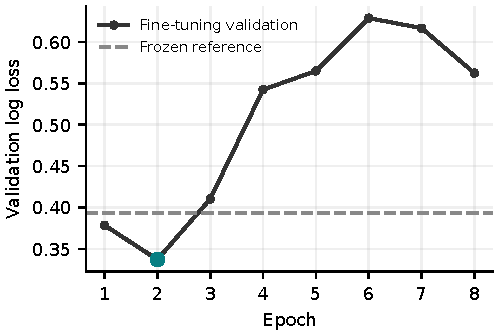
\includegraphics[width=\columnwidth]{figures/validation_loss.pdf}
\caption{Recorded validation log loss across the bounded fine-tuning run. The highlighted epoch 2 has the minimum loss. The dashed line is the original frozen reference.}
\label{fig:loss}
\end{figure}

\subsection{Fixed RWF evaluation}
Table~\ref{tab:evaluation} and Fig.~\ref{fig:rwfcm} compare both video models on all 400 RWF evaluation clips. Frozen accuracy is 84.0\% and fine-tuned accuracy 83.75\%. Fine-tuning increases Fight recall from 78.5\% to 87.5\% and AUC from 0.900 to 0.929. It reduces misses from 43 to 25 but increases false alarms from 21 to 40. With 200 clips per class, the false-positive rate changes from 10.5\% to 20.0\%, and the missed-Fight rate changes from 21.5\% to 12.5\%.

The selected candidate therefore exchanges 18 fewer misses for 19 more false alarms. Macro-F1 changes from 0.840 to 0.837, and violent precision decreases from 88.2\% to 81.4\%. Improved score ranking and recall do not require improved thresholded accuracy. Because thresholds are 0.50 and 0.23, the comparison combines parameter adaptation with a changed operating point. No additional threshold is tuned on these results.

\begin{table*}[t]
\caption{Fixed all-clip evaluation. Fight is positive. FP counts nonviolent clips flagged violent, and FN counts missed violent clips.}
\label{tab:evaluation}\centering
\begin{tabular}{llrrrrrrrrr}
\toprule
Set & Model & $n$ & $\tau$ & Accuracy & F1 & AUC & Precision & Recall & FP & FN\\
\midrule
RWF & Frozen video & 400 & 0.50 & 84.00\% & 0.840 & 0.900 & 88.2\% & 78.5\% & 21 & 43\\
RWF & Fine-tuned video & 400 & 0.23 & 83.75\% & 0.837 & 0.929 & 81.4\% & 87.5\% & 40 & 25\\
Hockey & Frozen video & 1000 & 0.50 & 70.80\% & 0.686 & 0.886 & 94.1\% & 44.4\% & 14 & 278\\
Hockey & Fine-tuned video & 1000 & 0.23 & 81.10\% & 0.810 & 0.893 & 86.6\% & 73.6\% & 57 & 132\\
Hockey & Crowd pose & 1000 & 0.62 & 40.90\% & 0.361 & 0.420 & 44.1\% & 68.2\% & 432 & 159\\
\bottomrule
\end{tabular}
\par\smallskip\parbox{\textwidth}{\footnotesize RWF results use previously inspected footage. All 1,000 Hockey mirror clips remain. The frozen video reference is the predeclared primary external model; fine-tuning is supplementary and crowd pose is diagnostic.}
\end{table*}

\begin{figure*}[t]
\centering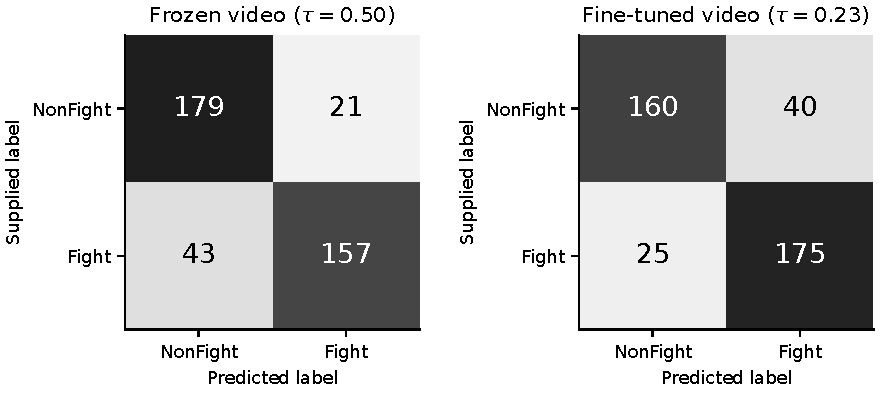
\includegraphics[width=.86\textwidth]{figures/rwf_confusion.pdf}
\caption{RWF all-clip confusion counts. Rows use supplied labels and columns use predictions. Fine-tuning at its validation-selected threshold reduces missed fights but increases false alarms.}
\label{fig:rwfcm}
\end{figure*}

\subsection{External hockey evaluation}
The fixed frozen RWF video model reaches 70.8\% accuracy on all 1,000 hockey clips. Its precision is 94.1\% but Fight recall only 44.4\%, with 278 misses and 14 false alarms. The supplementary fine-tuned model reaches 81.1\% accuracy and 73.6\% recall, with 132 misses and 57 false alarms. Its AUC is 0.893, compared with 0.886 for frozen video. Fig.~\ref{fig:external} illustrates the accuracy and recall differences.

The corrected crowd interactions checkpoint reaches 40.9\% accuracy, macro-F1 0.361, and AUC 0.420. It flags 432 of 500 nonviolent clips, while detecting 341 of 500 violent clips. Restricting to the 982 pose-supported clips gives 40.63\% accuracy and does not rescue performance. Poor support is therefore insufficient to explain the external failure. Sports-domain geometry, tracking behavior, threshold transfer, and missing context remain possible contributors, without a causal attribution from this experiment.

\begin{figure}[t]
\centering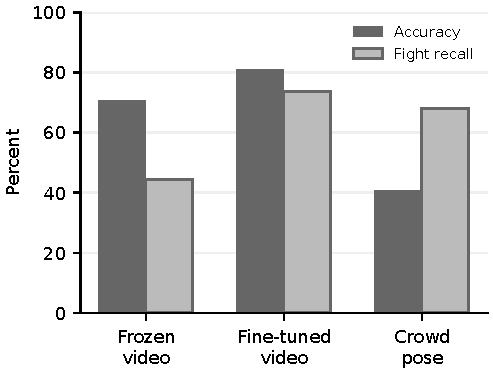
\includegraphics[width=\columnwidth]{figures/external_results.pdf}
\caption{All-clip Hockey Fight accuracy and Fight recall for fixed models. The video models were fitted on RWF, while the pose checkpoint was fitted on crowd footage.}
\label{fig:external}
\end{figure}

\subsection{Diagnostic clips and measured runtime}
Four final video examples cover true-positive, true-negative, false-positive, and false-negative outcomes relative to supplied labels. They are the most confident available examples in their confusion categories, selected after scoring for explanation. Each saved five-second MP4 contains 150 frames, fully decodes, and reproduces its stored score with zero observed drift. This verifies the saved demonstration and is not an independent accuracy sample.

Fig.~\ref{fig:failures} shows two error examples. The false-positive score is 0.999659 and the false-negative score 0.004315 at threshold 0.23. Neither the extremity of a score nor the appearance of one frame establishes correct labeling or explains the failure mechanism. These scores also show why the classifier output should not be presented as calibrated incident probability.

\begin{figure*}[t]
\centering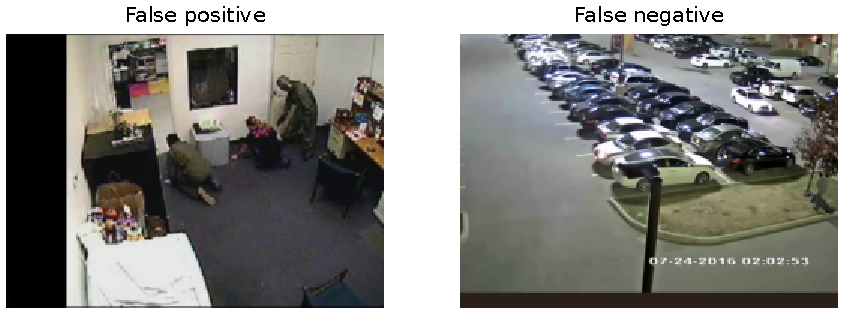
\includegraphics[width=.94\textwidth]{figures/failure_examples.pdf}
\caption{Frames cropped from saved RWF diagnostic videos. Left: supplied nonviolent label, violent prediction, score 0.999659. Right: supplied violent label, nonviolent prediction, score 0.004315. These outcome-selected examples illustrate disagreement with unreviewed supplied labels, not independently verified ground truth.}
\label{fig:failures}
\end{figure*}

Table~\ref{tab:runtime} gives warm pose-pipeline median 0.270 s and p95 0.390 s. Cold external-process median is 8.359 s and p95 8.503 s. Warm median pose/tracking time is 0.2408 s, whereas classifier time is 0.00246 s, illustrating why model-only timing would misrepresent the full pipeline. Component medians need not sum to the median of total time. Fig.~\ref{fig:runtime} shows individual recorded measurements with separate units for warm and cold boundaries.

The eight-epoch fine-tuning run takes 327.32 s and records peak PyTorch allocated GPU memory of 621,134,848 bytes, approximately 0.62 GB in decimal units. This is an allocator measurement, not total device memory. These training and pose-inference measurements do not establish fine-tuned RGB streaming speed or throughput.

\begin{table}[t]
\caption{Offline pose timing on ten fixed clips. Overlay generation and export are excluded.}
\label{tab:runtime}\centering
\begin{tabular}{lrr}
\toprule
Measurement & Median (s) & p95 (s)\\
\midrule
Warm pipeline (30 runs) & 0.270 & 0.390\\
Cold external process (10) & 8.359 & 8.503\\
\bottomrule
\end{tabular}
\end{table}

\begin{figure*}[t]
\centering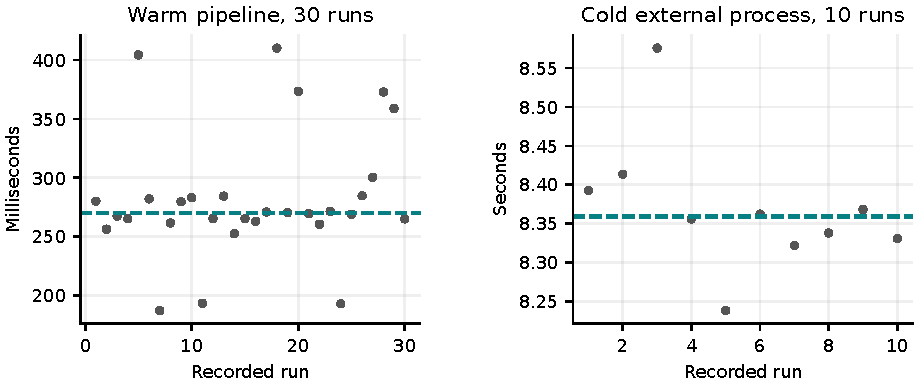
\includegraphics[width=.93\textwidth]{figures/runtime_runs.pdf}
\caption{Recorded pose timing. Warm values include the pipeline with loaded models; cold values include an external Python process and initialization. Axes use different units and scales. Dashed lines show medians. Overlay/export is excluded.}
\label{fig:runtime}
\end{figure*}
